\documentclass[a4paper]{article}
\usepackage{svg}
\usepackage{vntex}
\usepackage{pdflscape}
\usepackage{subcaption}
\usepackage{rotating}
\usepackage{a4wide,amssymb,epsfig,latexsym,multicol,array,hhline,fancyhdr}
\usepackage{minted}
\usepackage{booktabs}
\usepackage{float}
\usepackage{longtable}
\usepackage{placeins}
\usepackage{capt-of}
\usepackage{tabularx}
\usepackage{caption}
\usepackage{amsmath}
\usepackage{lastpage}
\usepackage{enumerate}
\usepackage{color}
\usepackage{graphicx}
\usepackage{multirow}
\usepackage[framemethod=tikz]{mdframed}
\usepackage{wrapfig}
\usepackage{geometry}
\usepackage{setspace}
\usepackage{tikz}
\usepackage{listings}
\usetikzlibrary{arrows,snakes,backgrounds,positioning,shapes}
\usepackage{hyperref}
\usepackage{indentfirst}
\usepackage{cases}
\usepackage{algorithm}
\usepackage{algpseudocode}
\usepackage{xcolor}
\usepackage[most]{tcolorbox}
\usepackage[shortlabels]{enumitem}

\renewcommand{\baselinestretch}{1.5}
\renewcommand{\figurename}{Hình}
\definecolor{termBG}{HTML}{0C1C23}
\definecolor{termWhite}{HTML}{F8F8F2}

\lstset{
    language=C,
    basicstyle=\ttfamily\footnotesize,
    numbers=left,
    numberstyle=\tiny,
    stepnumber=1,
    numbersep=5pt,
    backgroundcolor=\color{gray!10},
    keywordstyle=\color{blue}\bfseries,
    commentstyle=\color{green!50!black},
    stringstyle=\color{red},
    frame=single,
    breaklines=true,
}

\newtcbox{\code}{on line, 
    arc=2pt,                % Độ bo tròn góc
    colback=gray!20,        % Màu nền (xám nhạt)
    colframe=gray!20,       % Viền cùng màu nền
    boxrule=0pt,            % Không độ dày viền
    boxsep=0pt, left=2pt, right=2pt, top=2pt, bottom=2pt, % Khoảng cách đệm
    fontupper=\ttfamily     % Font chữ kiểu code
}

\newtcolorbox{softbox}{
    colback=black!3,        % Màu nền: Xám rất nhạt (3% đen)
    colframe=black!3,       % Màu viền: Trùng màu nền (để không thấy viền)
    arc=8pt,                % Độ bo tròn góc
    boxrule=0pt,            % Độ dày viền = 0
    left=10pt, right=10pt, top=8pt, bottom=8pt, % Khoảng cách lề bên trong
    fontupper=\itshape\color{black!80} % Font chữ: Nghiêng và màu xám đậm (80% đen)
}

\definecolor{codegreen}{rgb}{0,0.6,0}
\definecolor{codegray}{rgb}{0.5,0.5,0.5}
\definecolor{codepurple}{rgb}{0.58,0,0.82}
\definecolor{backcolour}{rgb}{0.95,0.95,0.92}

\definecolor{termBG}{HTML}{0C1C23}    % Màu nền xanh đen đậm
\definecolor{termRed}{HTML}{FF5555}   % Màu đỏ
\definecolor{termYellow}{HTML}{F1FA8C}% Màu vàng
\definecolor{termWhite}{HTML}{F8F8F2} % Màu chữ trắng sáng
\definecolor{termGray}{HTML}{A9B7C6}  % Màu xám nhạt (nếu cần)

\lstdefinestyle{terminalstyle}{
    basicstyle=\ttfamily\scriptsize\color{termWhite},
    backgroundcolor=\color{termBG},
    breaklines=true,
    columns=fullflexible,
    keepspaces=true,
    showstringspaces=false,
    frame=single,
    rulecolor=\color{termBG},
    framesep=4pt,
    numbers=none
}

% Lệnh tắt để tô màu cho nhanh
\newcommand{\cred}[1]{\textcolor{termRed}{#1}}
\newcommand{\cyellow}[1]{\textcolor{termYellow}{#1}}

% Cấu hình style cho C/C++
\lstdefinestyle{mystyle}{
    backgroundcolor=\color{backcolour},   
    commentstyle=\color{codegreen},
    keywordstyle=\color{magenta},
    numberstyle=\tiny\color{codegray},
    stringstyle=\color{codepurple},
    basicstyle=\ttfamily\footnotesize, % Font chữ kiểu máy đánh chữ, kích thước nhỏ
    breakatwhitespace=false,         
    breaklines=true,                 % Tự động xuống dòng nếu quá dài
    captionpos=b,                    
    keepspaces=true,                 
    numbers=left,                    % Hiển thị số dòng bên trái
    numbersep=5pt,                  
    showspaces=false,                
    showstringspaces=false,
    showtabs=false,                  
    tabsize=2,                       % Độ rộng tab = 2 spaces
    language=C                       % Ngôn ngữ mặc định
}

\lstset{style=mystyle}

\hypersetup{
    colorlinks=true,
    linkcolor=black,      % Màu link nội bộ (mục lục, cross-reference)
    citecolor=red,        % Màu citation (references)
    urlcolor=blue,        % Màu URL
    filecolor=magenta     % Màu link file
}

\setlength{\headheight}{40pt}
\pagestyle{fancy}
\fancyhead{} % clear all header fields
\fancyhead[L]{
 \begin{tabular}{rl}
    \begin{picture}(25,15)(0,0)
    \put(0,-8){
\includegraphics[width=8mm, height=8mm]{images/khtn.png}}
    \end{picture}&
	\begin{tabular}{l}
		\textbf{\bf \ttfamily Ho Chi Minh University of Science - VNUHCM}\\
		\textbf{\bf \ttfamily Faculty of Information Technology}
	\end{tabular}  	
 \end{tabular}
}
\fancyhead[R]{
	\begin{tabular}{l}
		\tiny \bf \\
		\tiny \bf 
	\end{tabular}  }
\fancyfoot{} % clear all footer fields
\fancyfoot[L]{\scriptsize \ttfamily Operating Systems}
\fancyfoot[R]{\scriptsize \ttfamily Page {\thepage}}
\renewcommand{\headrulewidth}{0.3pt}
\renewcommand{\footrulewidth}{0.3pt}

\setcounter{secnumdepth}{4}
\setcounter{tocdepth}{3}
\makeatletter
\newcounter {subsubsubsection}[subsubsection]
\renewcommand\thesubsubsubsection{\thesubsubsection .\@alph\c@subsubsubsection}
\newcommand\subsubsubsection{\@startsection{subsubsubsection}{4}{\z@}%
                                    {-3.25ex\@plus -1ex \@minus -.2ex}%
                                    {1.5ex \@plus .2ex}%
                                    {\normalfont\normalsize\bfseries}}
\newcommand*\l@subsubsubsection{\@dottedtocline{3}{10.0em}{4.1em}}
\newcommand*{\subsubsubsectionmark}[1]{}
\makeatother

\definecolor{dkgreen}{rgb}{0,0.6,0}
\definecolor{gray}{rgb}{0.5,0.5,0.5}
\definecolor{mauve}{rgb}{0.58,0,0.82}

\begin{document}

\begin{titlepage}
\begin{center}
VIETNAM NATIONAL UNIVERSITY HO CHI MINH CITY\\
HO CHI MINH CITY UNIVERSITY OF SCIENCE \\
FACULTY OF INFORMATION TECHNOLOGY
\end{center}

\vspace{0.7cm}

\begin{figure}[h!]
\begin{center}

\includegraphics[width=5cm]{images/khtn.png}
\end{center}
\end{figure}

\vspace{0.5cm}

\begin{center}
\begin{tabular}{c}
\multicolumn{1}{c}{\textbf{{\normalsize FACULTY OF INFORMATION TECHNOLOGY}}}\\
~~\\
\hline
\\
\multicolumn{1}{c}{\textbf{{\Large LAB REPORT}}}\\
\\
\textbf{{\Large Lab 01: Xv6 User Programs}}\\
\\
\hline
\end{tabular}
\end{center}

\vspace{0.5cm}

\begin{table}[h]
\begin{tabular}{rrll}
\hspace{4.5cm} & \textbf{Instructor:} & \\
\hspace{4.5cm} & \textbf{Leader:} & Phuc-Khang Nguyen & 24120068\\
\hspace{4.5cm} & Members: & Minh-Trong Pham & 24120151\\
\hspace{4.5cm} &  & Trong-Nghia Hoang & 24120103\\
\hspace{4.5cm} &  &  & 
\end{tabular}
\end{table}

\vspace{2.5cm}

\begin{center} {\footnotesize Ho Chi Minh City, \today}
\end{center}
\end{titlepage}


\thispagestyle{empty}

\newpage
\renewcommand{\contentsname}{Table of Contents}
\renewcommand{\tablename}{Table}
\renewcommand{\figurename}{Figure}
\renewcommand{\refname}{References}
\renewcommand{\listfigurename}{List of Figures}
\renewcommand{\listtablename}{List of Tables}

\tableofcontents

\newpage

\renewcommand{\arraystretch}{1.3} % Adjust row height
\setcounter{page}{1}

\section{Concurrent Prime Sieve (primes.c)}

\subsection{Ý tưởng thiết kế và Mô hình hoạt động}
Chương trình hiện thực thuật toán Sàng Eratosthenes đồng thời (\textit{Concurrent Prime Sieve}) dựa trên mô hình xử lý luồng dữ liệu qua chuỗi đường ống dẫn (\textit{concurrent pipeline}). 

Ý tưởng kết hợp đường ống Unix (\textit{pipe}) với thuật toán sàng số nguyên tố xuất phát từ đề xuất mang tính nền tảng của Doug McIlroy --- nhà khoa học máy tính tại Bell Labs và là người phát minh ra khái niệm Unix Pipeline \cite{mcilroy1968coroutines, mcilroy1978unix}. Mô hình này đại diện cho kiến trúc tính toán dòng dữ liệu CSP (\textit{Communicating Sequential Processes}) được khởi xướng bởi C. A. R. Hoare \cite{hoare1978csp}, đồng thời vận dụng trực tiếp các cơ chế quản lý tiến trình và giao tiếp liên tiến trình (IPC) trong hệ điều hành xv6 \cite{xv6book, remzi2018ostep}.

\begin{figure}[H]
    \centering
    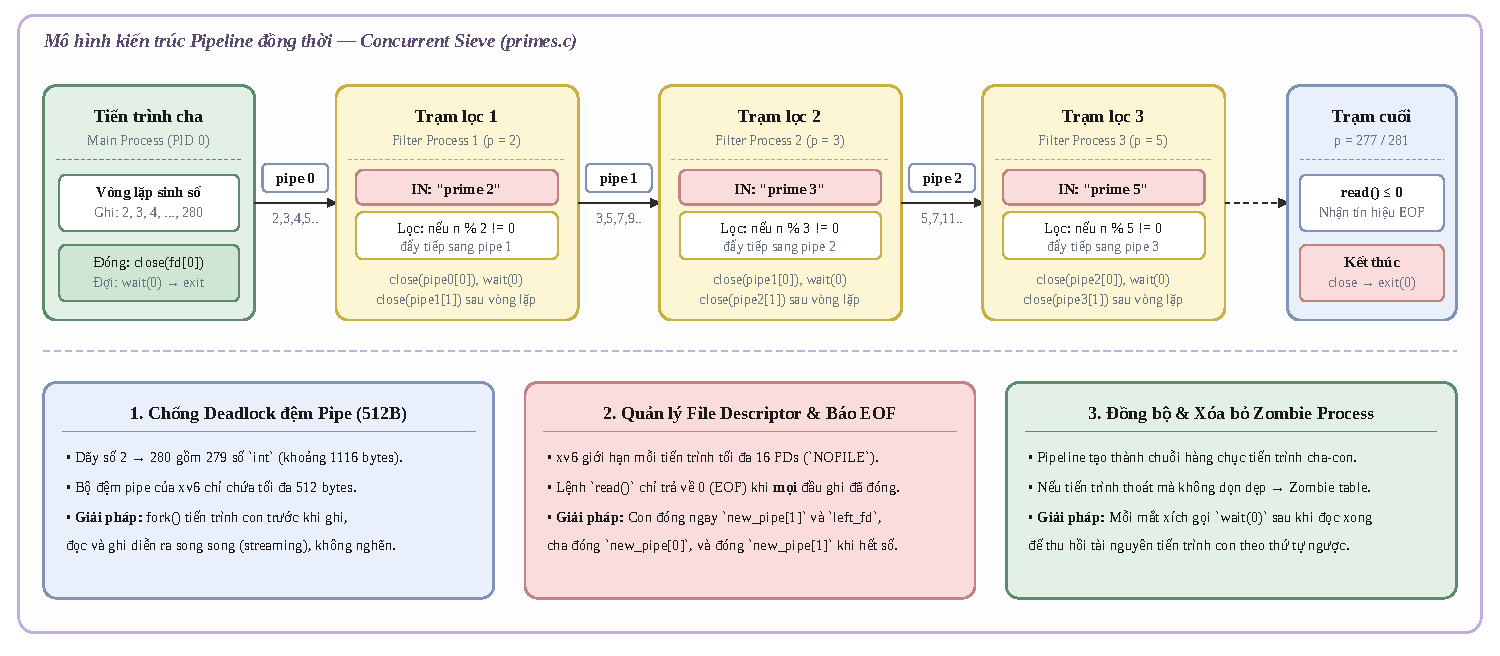
\includegraphics[width=\textwidth]{images/primes_pipeline.pdf}
    \caption{Mô hình luồng dữ liệu đường ống và các giải pháp hệ thống trong \texttt{primes.c}}
    \label{fig:primes_pipeline}
\end{figure}

\noindent Luồng thực thi diễn ra tuần tự qua các giai đoạn:
\begin{itemize}
    \item \textbf{Tiến trình khởi tạo (Main Process):} Tạo \code{pipe 0}, thực hiện \code{fork()} để tạo tiến trình con lọc đầu tiên, sau đó ghi dãy số từ $2$ đến $280$ vào đầu ghi của \code{pipe 0}.
    \item \textbf{Các trạm lọc trung gian (Filter Stages):} Mỗi tiến trình đọc số nguyên đầu tiên $p$ từ pipe bên trái (\code{left\_fd}). Số $p$ này chắc chắn là số nguyên tố và được in ra màn hình. Kế tiếp, tiến trình tạo một pipe mới (\code{new\_pipe}), \code{fork()} tiến trình con kế tiếp, rồi đóng vai trò lọc: đọc các số $n$ còn lại, nếu $n \pmod p \neq 0$ thì đẩy vào \code{new\_pipe}.
    \item \textbf{Trạm kết thúc (Termination):} Khi đường ống bên trái đóng hoàn toàn, hàm \code{read()} trả về giá trị $\le 0$ (EOF). Tiến trình thực hiện đóng đầu pipe, gọi \code{wait(0)} để đợi tiến trình con và thoát an toàn.
\end{itemize}

\subsection{Khó khăn kỹ thuật và Giải pháp thực tế}
Dựa trên các đặc thù kiến trúc và giới hạn tài nguyên của hệ điều hành xv6 \cite{xv6book}, bài làm đã giải quyết ba thách thức then chốt:
\begin{enumerate}
    \item \textbf{Ngăn ngừa Deadlock do bộ đệm Pipe giới hạn (512 bytes):} 
    Dãy số $2 \to 280$ tương ứng hơn $1.1\text{ KB}$ dữ liệu, vượt quá dung lượng đệm của một pipe trong xv6. Nếu tiến trình cha ghi toàn bộ dữ liệu trước khi con đọc, lời gọi \code{write()} sẽ bị chặn vô tận (\textit{blocked}) gây treo hệ thống. \\
    \textit{Giải pháp:} Khởi tạo \code{fork()} trước khi bắt đầu ghi, giúp luồng dữ liệu được tiêu thụ đồng thời dạng streaming.
    \item \textbf{Quản lý File Descriptor và tín hiệu ngắt EOF:}
    Hàm \code{read()} chỉ trả về 0 khi toàn bộ các đầu ghi của pipe đó được đóng. Nếu tiến trình con không đóng đầu ghi thừa kế thừa từ cha, lệnh \code{read()} sẽ chờ vĩnh viễn. Ngoài ra, xv6 giới hạn mỗi process chỉ có 16 FDs (\code{NOFILE}). \\
    \textit{Giải pháp:} Tiến trình con lập tức \code{close(new\_pipe[1])} và \code{close(left\_fd)}; tiến trình cha \code{close(new\_pipe[0])} và \code{close(new\_pipe[1])} ngay sau khi đẩy hết dãy số.
    \item \textbf{Thu dọn tài nguyên tiến trình con (Zombie Process):}
    Tất cả các tiến trình cha trong chuỗi đều gọi lệnh \code{wait(0)} trước khi kết thúc, đảm bảo bảng tiến trình của hệ điều hành được dọn dẹp sạch sẽ theo khuyến nghị quản lý tiến trình \cite{remzi2018ostep}.
\end{enumerate}

\newpage

\section{Directory Tree Visualization (tree.c)}

\subsection{Ý tưởng thiết kế và Cơ chế Lookahead Buffer}
Lệnh \code{tree} mô phỏng tiện ích dòng lệnh kinh điển trên hệ thống Unix/Linux do Steve Baker phát triển \cite{baker1996tree}. Chương trình duyệt hệ thống tệp đệ quy theo chiều sâu (DFS), hỗ trợ hiển thị cấu trúc phân nhánh đẹp mắt cùng các cờ tùy chọn \code{-L <depth>} (giới hạn độ sâu) và \code{-d} (chỉ hiển thị thư mục). Cấu trúc \texttt{struct dirent} và bảng chỉ mục \texttt{inum} được truy xuất trực tiếp từ hệ thống tệp tin xv6 \cite{xv6book}.

\begin{figure}[H]
    \centering
    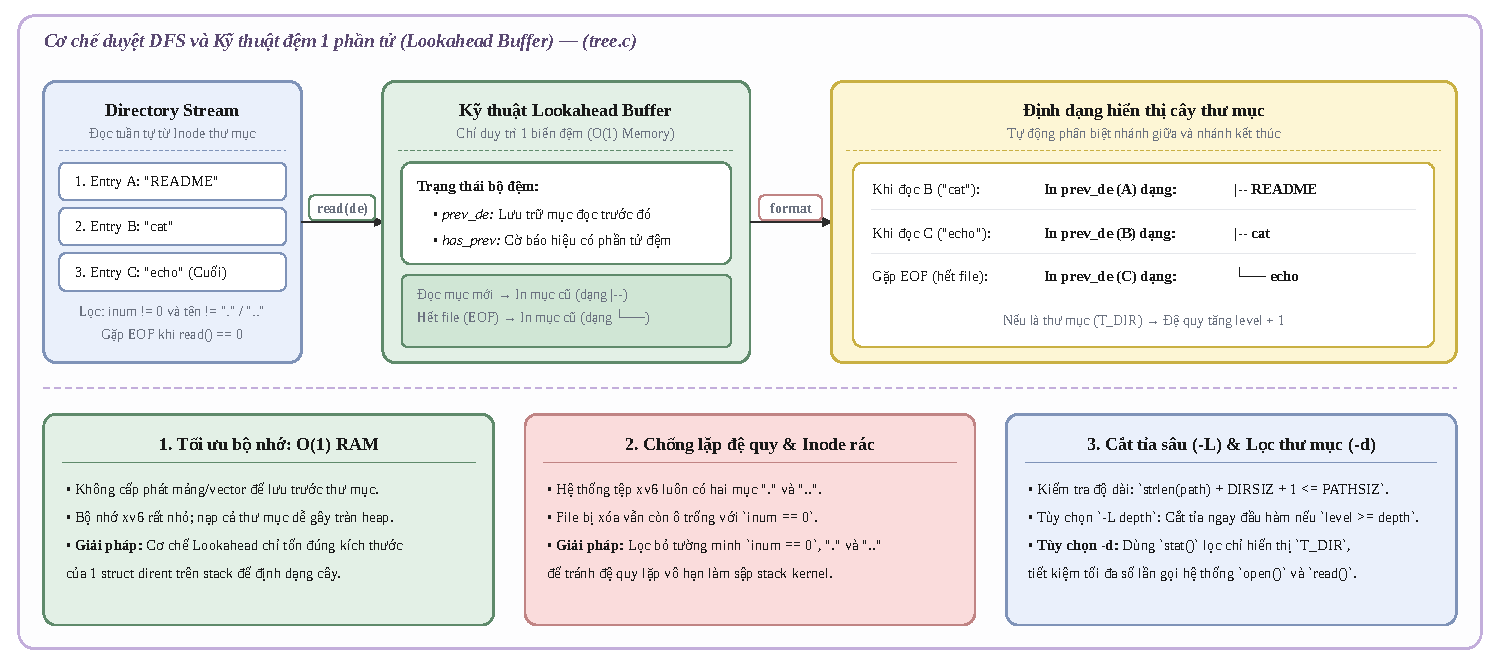
\includegraphics[width=\textwidth]{images/tree_lookahead.pdf}
    \caption{Cơ chế Lookahead Buffer $O(1)$ RAM và định dạng cây thư mục trong \texttt{tree.c}}
    \label{fig:tree_lookahead}
\end{figure}

\subsection{Điểm sáng giải thuật và Xử lý ca biên}
\begin{enumerate}
    \item \textbf{Kỹ thuật đệm 1 phần tử (1-Item Lookahead Buffer) đạt $O(1)$ bộ nhớ:}
    Để vẽ đúng định dạng cây chuẩn Unix (phần tử giữa dùng \texttt{|--}, phần tử cuối dùng \texttt{\textbackslash{}\_\_\_}), phương pháp thông thường cần nạp toàn bộ danh sách tệp vào mảng/vector để biết chỉ số cuối cùng. Trong môi trường nhúng có bộ nhớ hạn hẹp như xv6, giải pháp này dễ dẫn đến tràn bộ nhớ heap. \\
    \textit{Giải pháp:} Sử dụng bộ đệm chỉ gồm 1 phần tử (\code{prev\_de}, \code{prev\_stat}). Khi đọc một entry hợp lệ mới từ thư mục, chương trình mới in entry trước đó bằng ký hiệu \texttt{|--}. Khi gặp EOF (hết thư mục), entry đang nằm trong bộ đệm chắc chắn là phần tử cuối cùng và được in bằng \texttt{\textbackslash{}\_\_\_}.
    \item \textbf{Chống lặp đệ quy vô hạn và loại bỏ Inode rác:}
    Hệ thống tệp Unix luôn chứa hai liên kết đặc biệt là \texttt{"."} và \texttt{".."}. Chương trình chủ động lọc bỏ hai mục này và các ô inode trống (\code{inum == 0}) để bảo vệ stack kernel không bị tràn.
    \item \textbf{Kiểm soát độ dài đường dẫn và cắt tỉa đệ quy:}
    \begin{itemize}
        \item Kiểm tra an toàn trước khi ghép chuỗi: \code{strlen(path) + DIRSIZ + 1 <= PATHSIZ}.
        \item Tùy chọn \code{-L depth}: Dừng đệ quy sớm ngay từ điều kiện dừng (\textit{base case}) \code{level >= max\_depth}, tránh việc thực hiện lời gọi hệ thống \code{open()} không cần thiết.
        \item Tùy chọn \code{-d}: Dùng \code{stat()} kiểm tra kiểu inode (\code{T\_DIR}), lọc bỏ tệp tin ngay trong vòng lặp đọc.
    \end{itemize}
\end{enumerate}

\subsection{Kết quả thực nghiệm}
Chương trình hoàn thành xuất sắc các ca kiểm thử: chạy mặc định \code{tree}, giới hạn độ sâu \code{tree -L 2}, lọc thư mục \code{tree -d}, và chỉ định đường dẫn cụ thể mà không gặp bất kỳ lỗi rò rỉ bộ nhớ hay cạn kiệt file descriptor.


\newpage
\bibliographystyle{IEEEtran}
\bibliography{ref}
\end{document}
